\section[Interakce gamma záření]{Interakce gama záření s látkou, charakteristika gama spektra, charakteristiky a kalibrace detektorů}

\subsection{Základní poznatky}

\subsubsection{Zdroje fotonů}

Hlavním zdrojem gamma fotonů je RA rozpad částic (primárně $\beta$, pro vyšší $Z$ i $\alpha$). Nově vzniklá jádra jsou často ve vzbuzeném energetickém stavu a do základního stavu se vracejí vyzáření gamma fotonu o specifické energii a intenzitě. Tato energie je charakteristická pro daný izotop, a ačkoliv je gamma foton vyzářen nově vzniklým jádrem, v tabulkách se připisuje k původnímu nestabilnímu jádru (např. $^{90}$Sr se rozpadá na $^{90}$Y, gamma foton vyzáří $^{90}$Y, ale v tabulkách ho najdu u $^{90}$Sr). Tento proces je velmi rychlý (většinou do $10^{-12}$ s), pokud k němu dojde za delší dobu, tak se vzniklé izotopy označují jako \textbf{metastabilní stavy}.

Mimo to jsou s produkcí gamma fotonů spojeny další procesy související s RA rozpady:

\begin{itemize}
    \item $\beta^+$ rozpad -- vzniká pozitron, který je ihned zastaven v látce. Najde kamaráda elektron, čímž vzniká \textbf{pozitronium} (neboli krátce žijící vazba pozitronu a elektronu), anihiluje a vznikají 2 fotony o energii 511 keV jdoucí od sebe pod úhlem 180° (mohou vzniknout i 3 fotony, viz níže), tzv. \textbf{anihilační záření}. Jelikož před anihilací nezastaví pozitron uplně na nulu, je vzniklý peak rozmazaný.
    \item EC -- konkurenční k $\beta^+$, když není dostatek energie (<2$\times$ 511 keV), tak elektron potřebný ke konverzi protonu na neutron se vezme z obalu. Vzniká vakance v orbitale (nejčastěji K), která je zaplněna kaskádovými přeskoky z vyšších orbitalů, čímž vzniká charakteristické \textbf{RTG záření} (nebo Augerův elektron).
    \item IC -- neboli vnitřní konverze, vzbuzená jádra se mohou energie zbavit tak (kromě klasického $\gamma$ přechodu), že vnitřně předají energii elektronům v obale. Ten je uvolněn, vzniká vakance, která je opět kaskádami zaplněna za vzniku charakteristického \textbf{RTG záření} (nebo Augerova elektronu).
\end{itemize}

K tomu navíc existuje:

\begin{itemize}
    \item \textbf{okamžité záření} -- vzniká v důsledku jaderných reakcí, např. (n,$\gamma$), tedy gamma fotony uvolněné hned v rámci reakce, nikoliv následný rozpad (může přesahovat až 10 MeV).
    \item \textbf{brzdné záření} -- vzniká, pokud na nabitou částici působí zrychlení (zatáčí vlivem magnetického pole, k čemuž postačí Coulombovské pole vzbuzené jádrem), což je doprovázeno ztrátou energie ve formě brzdného záření. Záření je spojité a přispívá k nárůstu kontinua v gamma spektru. Záření je vyšší pro vyšší $Z$, proto by v oblasti detektoru měly být lehké materiály.
\end{itemize}

\subsubsection{Členění fotonů}

\begin{itemize}
    \item \textbf{RTG fotony} -- vznikají v orbitalech přeskoky elektronů. Energie je dána rozdílem energií orbitalů, což je dáno hlavním a vedlejším kvantovým číslem. Nicméně elektron nemůže skákat jen tak, řídí se Paulovým vylučovacím principem, který jasně říká, v jakém pořadí se elektrony zaplňují. Nižší energie, do desítek keV. Záření je čárové a charakteristické, ale ke každému izotopu existuje spoustu peaků, jelikož záleží na přesném módu přestupu (K$_{\alpha1}$, K$_{\alpha2}$ apod.).
    \item \textbf{Gamma fotony} -- vznikají deexcitací jádra. Opět čátové charakteristické záření, ale je zde výrazně méně možností (žádné módy). Energie je vyšší, až jednotky MeV.
    \item[-] V oblasti 1 MeV se fotony překrývají, členění není tak striktní.
\end{itemize}

\subsection{Interakce gamma záření s látkou}

Fotony jsou EM záření, kterému přísluší kvantum energie dle:

$$ E_\gamma = h \nu = h \dfrac{c}{\lambda}. $$

Vlnové délky se pohybují řádově $\lambda << 10^{-10}$ m, což je výrazně méně než meziatomové vzdálenosti v mřížce. Někdy se chová jako vlna (fotoefekt), jindy jako kulička (Comptonův rozptyl).

Jelikož nejde o nabité částice (tzv. \textbf{nepřímo ionizující záření}), tak se při detekci musí spoléhat na konverzi a detekují se až sekundární částice (elektrony).

Typ interakce je podmíněný energií (např. k tvorbě páru nedojde, je-li energie pod 1022 keV). 

\textbf{Koeficient zeslabení} = charakterizuje zeslabení způsobené absorbcí v daném materiálu (osa $y$) v závislosti na energii (osa $x$). Jde o součet křivek zeslabení způsobených fotoefektem, omptonovým rozptylem a tvorbou páru.

\textbf{Absorbční koeficient} = podíl energie pohlcené absorbčním materiálem při průchodu gamma záření, jelikož ne každá interakce vede na absorbci celé energie primárního fotonu.

\subsubsection{Primární interakce}

Máme 3 základní a nejdominantnější primární interakce: fotoefekt, Comptonův rozptyl a tvorba párů. Zbytek interakcí je z pohledu detekce zanedbatelný. Tím vznikají sekundární nabité částice (elektrony), které je možné detekovat.

Celkovou pravděpodobnost interakce (mikroskopický účinný průřez $\tau$, $\sigma$ a $\kappa$) je pak možné převést do \textbf{lineárního koeficientu zeslabení}, který vyjadřuje pravděpodobnost interakce na jednotku dráhy (makroskopický účinný průřez $\mu$). 

Z toho vychází i \textbf{střední volná dráha} $\lambda$:

$$ \lambda = \dfrac{1}{\mu}, $$

a \textbf{zeslabovací zákon}:

$$ \boxed{ \dfrac{I(x)}{I_0} = e^{-\mu x}. } $$

Pokud je vzorek emitující fotony tlustý (tloušťka $L$), dochází k samostnínění (část fotonů se pohltí) a celková intenzita se musí určit integrací:

$$ \boxed{ I_\gamma(L) = \dfrac{1}{L} \int_0^L I_\gamma^0 e^{-\mu x} \: \text{d}x = \dfrac{I_\gamma^0}{\mu L} \left( 1 - e^{-\mu L} \right).} $$

V tabulkách se pak uvádí \textbf{hmotnostní koeficient zeslabení}, který je svázaný s hustotou materiálu:

$$ \mu(\text{cm}^2{\text{/g}}) = \dfrac{\mu(\text{1/cm})}{\rho(\text{g/cm}^3)}. $$

\begin{figure}[H]
    \centering
    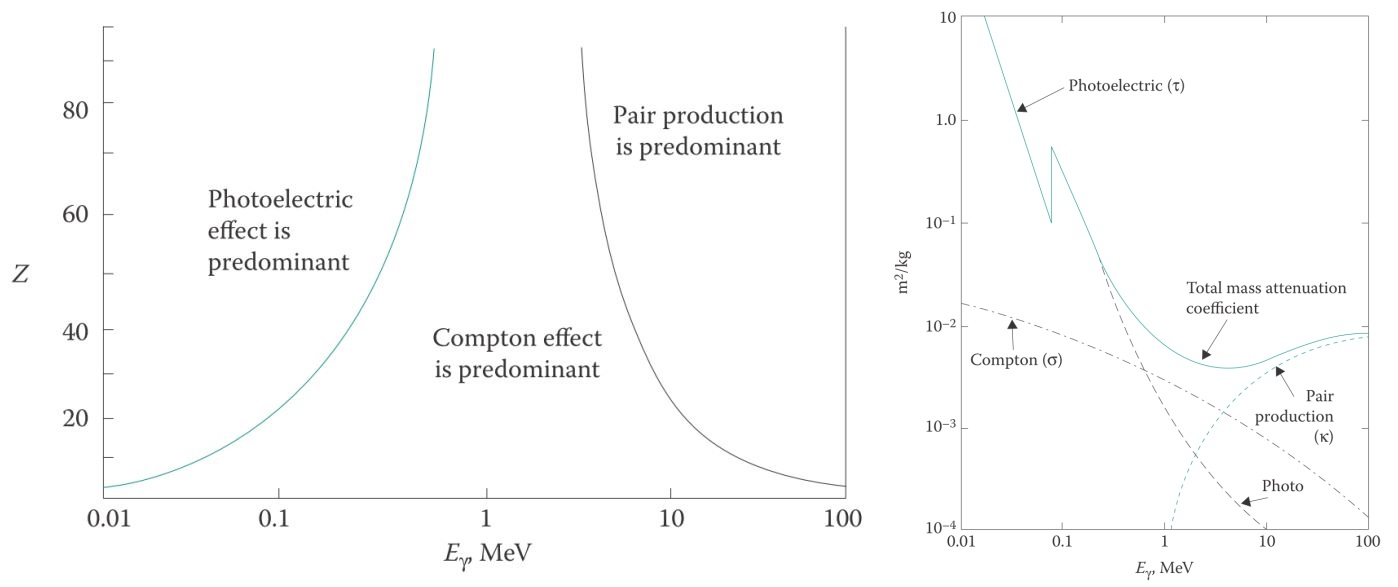
\includegraphics[width=1\textwidth]{img/interakce.JPG}
\end{figure}

\textbf{Fotoefekt:} jde o jev, kdy primární foton interaguje s elektronem v obalu, odevzdá mu veškerou svoji energii, foton zanikne a tzv. fotoelektron je uvolněn (energie fotonu $E_\gamma$ se rozdělí na vazebnou energii elektronu $E_b$ a kinetickou energii elektronu $E_e$):

$$ E_e = E_\gamma - E_b. $$

Jde o dominantní reakci při absorbci do 200 keV. Pravděpodobnost rekace (účinný průřez reakce $\tau$) klesá s energií $E_\gamma$ a roste se $Z$, jako:

$$ \tau = c \dfrac{Z^n}{E_\gamma^{3,5}}, \: \: \: n \in (4,5). $$

Energetické spektrum fotoelektronů (sekundární částice) je \textbf{čárové} a fotoefekt je zodpovědný za \textbf{fotopeak}. Fotoelektrony mohou být uvolněny z libovolného orbitalu (nejpravděpodobněji K orbital), nicméně při nižší energii než $E_{V_K}$ už foton není schopný vyrazit elektron z K orbitalu, $\tau$ skokově klesá a dochází k vyrážení z vyšších orbitalů.

\begin{figure}[H]
    \centering
    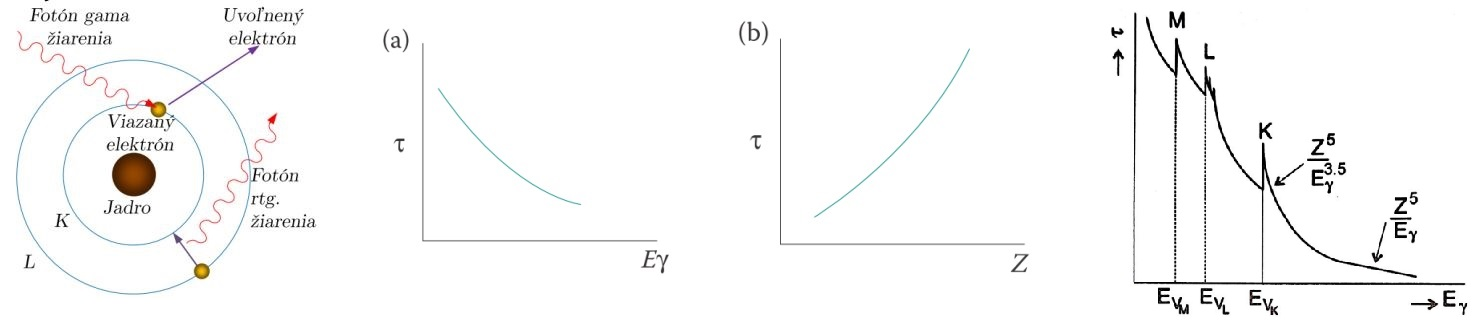
\includegraphics[width=1\textwidth]{img/fotoefekt.JPG}
\end{figure}

\textbf{Comptonův rozptyl:} jde o rozptyl fotonů na atomovém obale. Foton se odrazí od elektronu pod úhlem $\theta$ s novou energií (resp. vlnovou délkou) dle vztahu:

$$ E_\gamma' = \dfrac{E_\gamma}{1 + \dfrac{E_\gamma}{m_\text{e}c^2}(1 - \text{cos}(\theta))}. $$

Dochází k němu pro vyšší energie, pokud je energie nalétávajícího fotonu vyšší, než vazebná energie elektronu v obalu. Pravděpodobnost interakce (účinný průřez $\sigma$) je úměrná $Z$ a nepřímo úměrná energii $E_\gamma$:

$$ \sigma \sim \dfrac{Z}{E_\gamma}. $$

Tím vznikají odražené elektrony (sekundární částice), které jsou detekovány. Energetické spektrum odražených elektronů je \textbf{spojité}, tzv. \textbf{Comptonovo kontinuum}. To je zakončeno \textbf{Comptonovou hranou}, která je dána maximální energií elektronů (k tomu dojde, dojde-li k čelní srážce, kdy $\theta = 180°$).

Úhlová distribuce rozptýlených fotonů je dána Klein-Nishinovým vztahem pro diferenciální účinný průřez, s rostoucí energií gamma fotonů roste pravděpodobnost dopředných úhlů.

\begin{figure}[H]
    \centering
    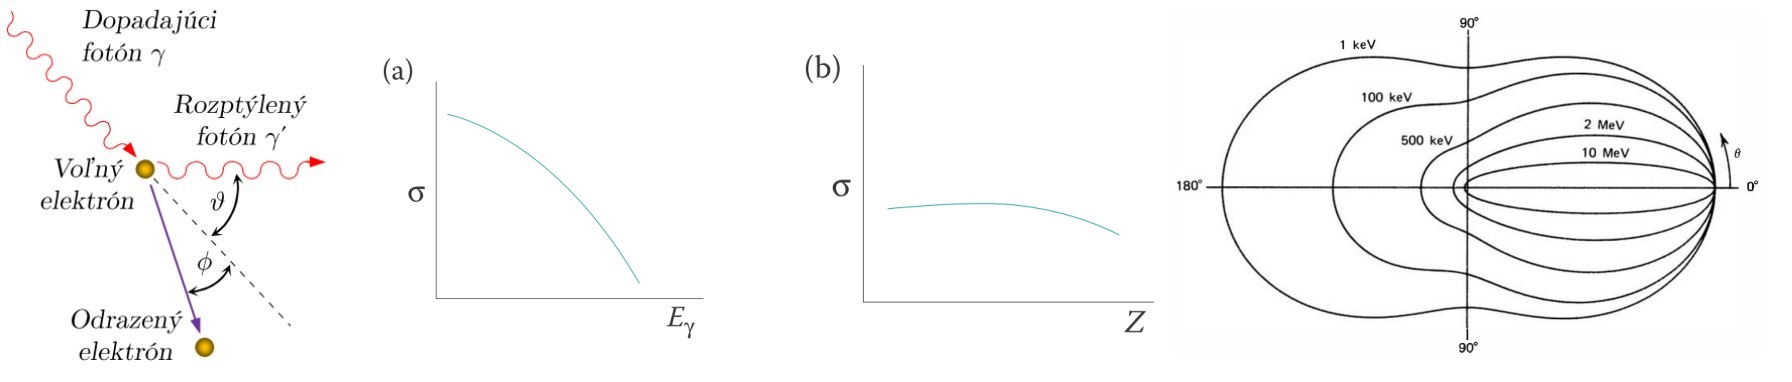
\includegraphics[width=1\textwidth]{img/Compton.JPG}
\end{figure}

\textbf{Tvorba elektron-pozitron páru:} jde o důsledek interakce gamma fotonu s jádrem atomu. Dojde k zaniknutí gamma fotonu a vznikne pár elektron-pozitron o energiích:

$$ E = \dfrac{1}{2} (E_\gamma - 1022 \text{ keV}). $$

Elektron i pozitron se ihned zastaví a v případě pozitronu dojde ke vzniku pozitronia, anihilaci a vzniku 2-3 fotonů.

Pravděpodobnost interakce (účinný průřez $\kappa$) roste s energií $E_\gamma$ a je přímo úměrná $Z^2$. Zároveň jde o prahovou reakci a je dominantní pro vysoké energie:

$$ \kappa \sim Z^2 \: \text{ln} \left( \dfrac{E_\gamma}{m_\text{e} c^2} \right). $$

\begin{figure}[H]
    \centering
    \includegraphics[width=0.7\textwidth]{img/pár.JPG}
\end{figure}

\textbf{Fotojaderné reakce:} při interakci a pohlcení gamma fotonů může být z jádra emitován nukleon.

Jde o prahové reakce a je jich spousta: ($\gamma$,n), ($\gamma$,2n), ($\gamma$,p), ($\gamma$,np), ($\gamma$,$\alpha$) apod. Jde o prahové reakce (alespoň 5 MeV), v porovnání s předchozími 3mi reakcemi jsou zanedbatelné. Problematické v radiační ochraně (emitují se těžké nabité částice).

V JI se využívají hlavně k emitování neutronů, jako fotojaderné neutronové zdroje (např. $^{206}$Pb, $^{9}$Be, $^2$H, $^{7}$Li, $^{14}$N apod.)

\textbf{Rayligho rozptyl:} jde o koherentní rozptyl fotonu s celým obalem (tedy se všemi elektrony), přičemž nedochází k ionizaci, ani excitaci (nepřenáší se enegie, vlnová délka fotonů se zachovává). Pouze se mění směr hybnosti fotonů.

Opět nepříliš dominantní interakce, lze zanedbat. Roste pro nízké energie fotonů a vysoká $Z$. Vsuvka, vysvětluje, proč je obloha modrá (ale nevim proč :D).

\subsubsection{Druhotné efekty}

V případě detekce může docházet k zaznamenávání nechtěných druhotných efektů.

\textbf{Vícenásobná interakce:} Comptonovsky rozptýlené fotony v citlivé oblasti detektoru mohou znovu interagovat (fotoefektem, Comptonovsky), což může přispět do peaku úplné absorbce, nebo vytvořit novou Comptonovu hranu.

\textbf{Peak zpětného rozptylu:} fotony proletí detektorem bez interakce, Comptonovsky interagují až v okolním materiálu, rozptýlí se zpět s nižší energií do citlivé oblasti detektoru a jsou zaregistrovány. Tím vzniká peak zpětného rozptylu s nižší energií.

\textbf{Anihilace elektron-pozitron:} pokud mimo detektor dojde ke tvorbě páru, vzniklý elektron a pozitron za vzniku pozitronia anihilují a jeden z fotonů se dostane zpět do detektoru. Absorbcí fotoefektem vzniká anihilační peak 511 keV.

\textbf{Pozitronium} je vázaný systém, analogický atomu vodíku, kdy elektron a pozitron obíhají kolem společného těžiště s dobou života okolo 10$^{-10}$. Existují 2 typy v závislosti na spinu:

\begin{itemize}
    \item Para-pozitronium -- spiny opačně, vznikají 2 fotony o energii 511 keV (dominantní),
    \item Orto-pozitronium -- spiny shodně, vznikají 3 fotony (málo časté).
\end{itemize}

\textbf{RTG záření:} je způsobené fotoefektem, kdy je vzniklá vakance zaplněna jiným elektronem a vyzářením RTG záření.

\textbf{Augerovy elektrony:} konkurenční proces k RTG záření, pouze je přebytečná energie předána sousednímu elektronu, který je uvolněn a vyletí ven.

\textbf{Brzdné záření:} vzniká, pokud elektrony a pozitrony proletí kolem jádra, které vyvolává Coulombovo EM pole.

\textbf{Sumační efekty:} ovlivněno geometrií detektoru, můžou být zaznamenány 2 gamma kvanta ve stejný okamžik (např. 511 keV + gamma deexcitace)

\textbf{Pozadí:} detektor detekuje záření z přirozeného prostředí, jde hlavně o izotopy $^{40}$K, $^{137}$Cs a produkty rozpadových řad (urany, radony apod.). Lze zamezit dobrým stíněním.

\subsection{Charakteristika gamma spektra}

\subsubsection{Tvar gamma spektra}

Spektrum, které zaznamenám, je dáno vlastnostmi detektoru.

\textbf{Limitní případ malého detektoru:} nastává, pokud střední volná dráha sekundárních fotonů (řádově jednotky cm) je výrazně větší, než citlivá plocha detektoru (do 1-2 cm). Detektor tak zaznamená pouze primární interakce, nedochází k vícenásobné interakci. Sekundární fotony vyletí ven.

Za předpokladu, že detektor zaznamená veškerou energii sekunádrních elektronů, tak se spektrum projeví Comptonovým kontinuem zakončeným Comptonovou hranou (Comptonův rozptyl) a fotopeakem úplné absorbce (fotoefekt, vznikne \textbf{FEP = Full Energy Peak}). 

Pro energie větší než 1022 keV se navíc projeví efekt tvorby párů (vznikne \textbf{DEP = Double Escape Peak}), anihilační fotony (jde o sekundární fotony) uniknou.

$$ E_\text{DEP} = E_\text{FEP} - 2 \cdot 511 \text{ keV}. $$

\begin{figure}[H]
    \centering
    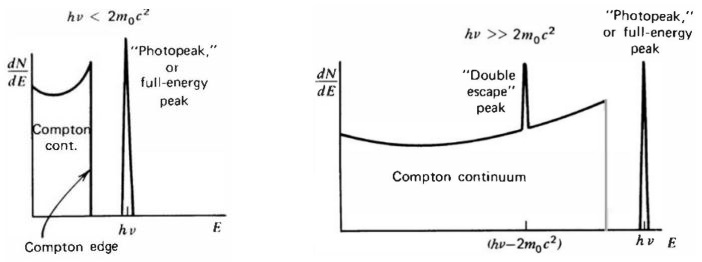
\includegraphics[width=0.7\textwidth]{img/maly_detektor.JPG}
    \caption{Tvar gamma spektra pro malý detektor ($E_\gamma < 1022$ keV vlevo, $E_\gamma > 1022$ keV vpravo).}
\end{figure}

\textbf{Limitní případ velkého detektoru:} pokud je střední volná dráha sekundárních fotonů výrazně menší, než rozměry detektoru. Ten pak zaznamená veškeré interakce, nic neunikne. Nakonec pak vždy dojde k fotoabsorbci, veškerá energie primárního záření je doponována v detektoru, tudíž zaznamenaný náboj sekundárních elektronů odpovídá energii primárního záření. Výsledná odezva je stejná, jako by primární gamma záření interagovalo pouze fotoefektem.

Spektrum se projevuje pouze peakem úplné abosrbce FEP, v tomto případě \textbf{peak úplného pohlcení}.

\begin{figure}[H]
    \centering
    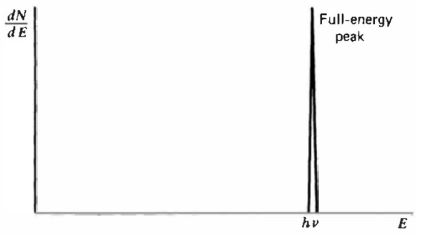
\includegraphics[width=0.4\textwidth]{img/velky_detektor.JPG}
    \caption{Tvar gamma spektra pro velký detektor.}
\end{figure}

\textbf{Středně velký detektor:} Ve skutečnosti vždy něco vylétne (kor, pokud dojde k reakci na kraji detektoru), tudíž reálný detektro zaznamená něco mezi. Nízkoenergetické záření se zaznamená lépe, jelikož nedochází tak často k sekundárním interakcím. Pak dochází k vícenásobným Comptonovým rozptylům, které vyplňují mezeru mezi Comptonovou hranou a fotopíkem.

Pro energie větší než 1022 keV se opět projevuje DEP, ale navíc i \textbf{SEP = Single Escape Peak} (pokud jeden foton unikne, a druhý ne).

$$ E_\text{SEP} = E_\text{FEP} - 511 \text{ keV}. $$

\begin{figure}[H]
    \centering
    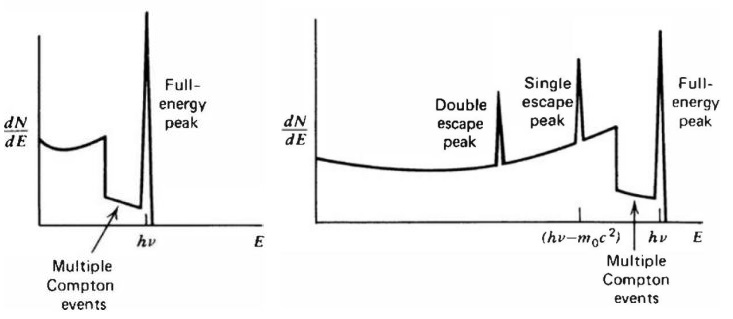
\includegraphics[width=0.7\textwidth]{img/stredni_detektor.JPG}
    \caption{Tvar gamma spektra pro středně velký detektor ($E_\gamma < 1022$ keV vlevo, $E_\gamma > 1022$ keV vpravo).}
\end{figure}

V každém případě nedojde k deponování veškeré energie a některé sekundární fotony uniknou, tento efekt nárůstá s energií těchto fotonů. To způsobuje zkreslení odezvové funkce a některé události jsou posunuty do nižších energií.

$\rightarrow$ \textbf{Ve zkratce.} Pokud mi nic neunikne, objeví se pouze FEP. Reálně ale něco unikne, což se projeví ve formě SEP a DEP (uniklé anihilační fotony). Pokud je detektor hodně malý, tak unikne vše sekundární a projeví se pouze DEP.

Ideálně chceme znát pouze FEP, přičemž Comptonovo kontinuum nám zkresluje měření. Pro jeho potlačení je možné využít koincidenční nebo antikoincidenční zapojení vícera detektorů a detekovat pouze určité interakce (v tomto případě FEP):

\begin{itemize}
    \item Comptonův spektrometr -- gamma-gamma spektrometr, mám 2 detektory pod úhlem $\theta$ a matematickým postprocessingem Comptonovo kontinuum eliminuju.
\end{itemize}

\subsubsection{Další efekty}

\textbf{RTG únikové peaky:} ty jsou způsobeny tím, že uniknou RTG fotony, které vzniknou kaskádou po fotoefektu (tzv. \textbf{XEP = X-ray Escape Peak}). V případě nekonečně velkého detektoru neuniknou a opět se veškerá energie deponuje v FEP.

$$ E_\text{XEP} = E_\text{FEP} - E_\text{X}. $$

\textbf{Anihilační peaky:} projeví se hlavně, je-li zářič $\beta^+$ radioaktivní. Pozitron anihiluje v materiálu a vzniknou gamma fotony o 511 keV. Pokud neuniknou, projeví se ve formě FEP na energii právě 511 keV. Pokud zaznamenáváme celou prostorovou geometrii, tak se projeví ve formě FEP na energii 1022 keV (zaznamenám oba dva najednou).

\textbf{Brzdné záření:} pokud máme gamma zářič $\beta$ radioaktivní, mohou unikat $\beta$ částice přímo ze zdroje a za vzniku brzdného záření zkreslovat spektrum. K tomu se používají filtry ($\beta$ absorbátory) z lehkých materiálů, které je pohltí (např. Be).

\textbf{Okolní materiály:} tvar gamma spektra a jeho zkreslení mohou ovlivňovat i okolní materiály, s kterými záření může interagovat (stínění, pouzdro, materiál zářiče, zpětně rozptýlené gamma, sumační peaky apod.)

\begin{figure}[H]
    \centering
    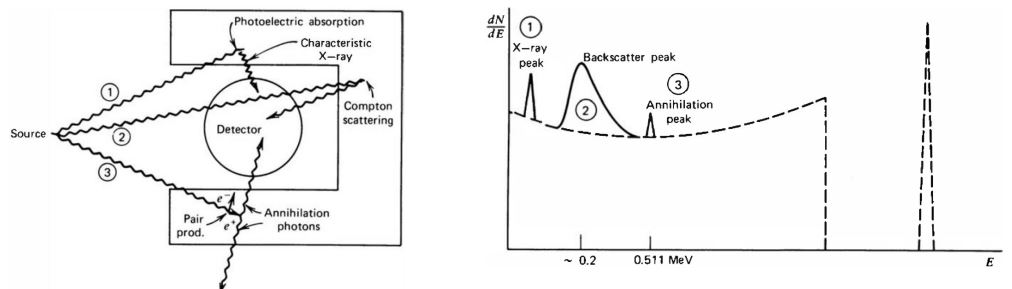
\includegraphics[width=0.9\textwidth]{img/vliv_materialu.JPG}
    \caption{Vliv okolních materiálů na tvar gamma spektra.}
\end{figure}

\subsubsection{Měření}

Při měření se projevuje statistika. My jsme v rámci detekce schopni zaznamenat histogramový záznam v jednotlivých energetických kanálech. Pod 100 zaznamenaných událostí je třeba uvažovat Poissonovo rozdělení, nad 100 událostí Gaussovo rozdělení (čas vs. aktivita). 

Ve výsledku poté zaznamenáme celkovou plochu pod peakem $S$ s potlačením Comptonova kontinua a pozadí pod peakem a s nejistotou, kterou určím z matematického popisu Gaussiánu. Dále se určí statistická významnost dle:

\begin{itemize}
    \item kritický limit $L_C$ -- plocha $S$ musí být větší než minimální hodnota,
    \item horní limit $L_U$ -- hodnota, kterou by plocha $S$ neměla překročit,
    \item detekční limit $L_D$ -- hodnota, nad kterou je plocha $S$ detekovatelná,
    \item limit stanovitelnosti $L_Q$ -- hodnota, nad kterou určím plochu $S$ s předem danou nejistotou.
\end{itemize}

$$ L_C < L_D < L_Q < S < L_U $$

\textbf{MDA} = Minimální detekovatelná aktivita, jde o nejmenší aktivitu, které může být s jistoutou měřené.

\subsection{Detektory gamma záření}

\subsubsection{Základní typy detektorů}

\textbf{Scintilační detektory:}

\begin{itemize}
    \item[1)] Primární gamma záření putuje do scintilačního krystalu, absorbuje se a část záření se transformuje na záblesk viditelného světla (\textbf{luminiscence}, atomy jsou excitovány a deexcitují viditelnými fotony), energie je úměrná světelnému signálu.
    \item[2)] Fotony putují fotonásobičem (elektronka), který mění světlo na elektrický signál. Ve formě fotokatody na vstupu, ze které jsou fotoefektem emitovány elektrony (to je ten signál).
    \item[3)] Na výstupu je anoda a vzniklé napětí urychluje elektrony za vzniku elektrického proudu. elektrony postupně dopadají na dynody, na kterých jsou vyráženy nové elektrony (2-6) a signál je zesilován. Je možné zesílit intenzitu elektronů až o 5 řádů.
    \item[4)] Takto zesílený proud je již detekovatelný, je vyveden na pracovní odpor, na kterém se mění napětí (to je ten signál, který měřím). 
\end{itemize}

\begin{figure}[H]
    \centering
    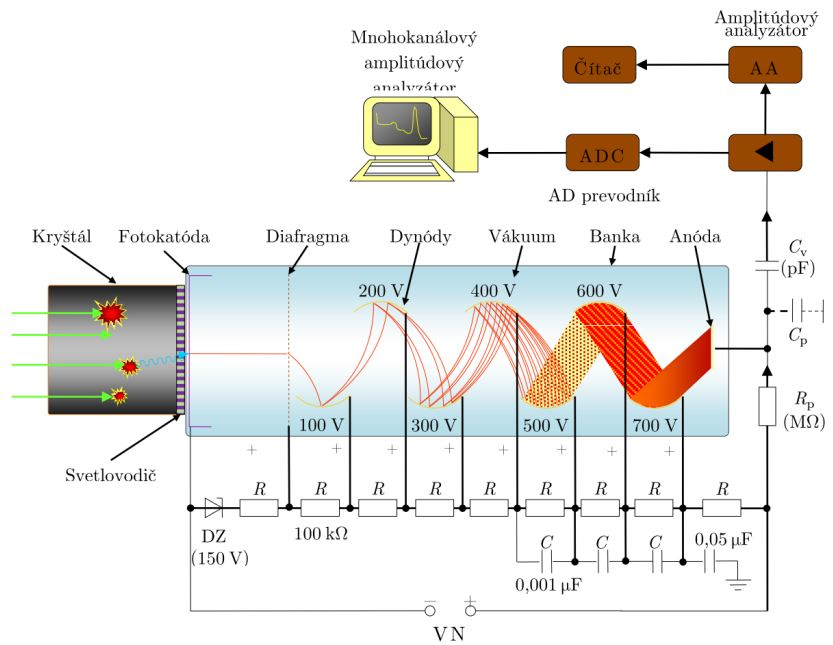
\includegraphics[width=0.65\textwidth]{img/scintilak.JPG}
    \caption{Princip scintilačního detektoru.}
\end{figure}

Scintilační krystal může být:

\begin{itemize}
    \item \textbf{Anorganický} -- primárně pro spektrometrii (gamma). 
    \item[-] Krystal je tvořen nejčastěji alkalickými kovy s malou příměsí nečistoty (tzv. aktivátor, to co je v závorce a ten je zodpovědný za luminiscenci): NaI(Tl), CsI(Tl), CaI(Na), LiI(Eu), CaF$_2$(Eu). 
    \item[-] Pro nízkoenergetické je lepší krystal s malým $Z$, pro vysokoenergetické s velkým $Z$ (ale tam je potom menší energetická rozlišitelnost).  
    \item \textbf{Organický} -- primárně pro neutrony a nabité částice.
    \item[-] Krystal je tvořen organickými molekulami na bázi benzenu a luminiscence je způsobena molekulárními deexcitacemi.
    \item[] Mohou být krystaly (antracen), kapaliny (rozpouštědlo + org. aktivátor, např. toluen + p-terphenyl), plasty (org. aktivátor v polymeru)
\end{itemize}

\textbf{Polovodičové detektory:}

\begin{itemize}
    \item[1)] Ve formě diody z čistého polovodiče v závěrném směru. Gamma záření způsobuje vyrážení elektronů, které se dostávají do vodivého pásma.
    \item[2)] Vznikají tak páry elektron-díra, které jsou nosičemi náboje, čímž vzniká elektrický signál.
    \item[3)] Ten putuje do předzesilovače, zesilovače, tvaruje se a zaznamenává v MCA.
\end{itemize}

Mají mnohem lepší energetickou rozlišitelnost, ale jsou dražší a musejí se chladit (jinak elektrony vyskakují samy a vzniká tak šum). Momentálně nejlepším detektorem je superčistý krystal germania (HPGe).

\textbf{Rozdíly:} polovodičové detektory mají lepší energetickou rozlišitelnost, ale menší detekční účinnost. Také jsou levnější.

\subsubsection{Základní charakteristiky}

\textbf{Odeva detektoru:} poměr mezi energií záření a pozorovaným výstupem (binem) na detektoru (záření o energii $E$ vytvoří $N$ nosičů náboje, které způsobí napěťový rozdíl na elektrodách detektoru, což je to, co detektor zaznamená).

\textbf{Odezvová funkce:} vyjadřuje pravděpodobnost, že monoenergetické fotony budou zaznamenané v daném energetickém binu.

\textbf{Časová odezva detektoru:} čas potřebný k vytvoření signálu. Signál je ve tvaru ostré náběžné a pozvolné seběžné hrany.

\textbf{Časové rozlišení:} nejmenší časová rozlišitelnost mezi dvěmi signály.

\textbf{Citlivost detektoru:} schopnost detektoru produkovat měřitelný signál pro konkrétní typ částice s danou energií. závisí na účinných průřezech, rozměrech hmotnosti, materiálech, šumu (ten může růst s rostoucím rozměrem detektoru).

\textbf{Mrtvá doba:} čas potřebný na zpracování signálu.

\textbf{Energetické rozlišení} nejmenší energetická rozlišitelnost mezi dvěmi signály. Detektor s dobrým rozlišením má užší a vyšší peak, než detektor s horším rozlišením (ale plochy pod peakem jsou stejné).

\textbf{FWHM} = Full Width at Half Maximum, stanovuje šířku pulzu (peaku) v polovině jeho maxima. Dáno energetickým rozlišením. Z toho je možné stanovit relativní energetické rozlišení jako:

$$ R = \dfrac{\text{FWHM}}{E}. $$

Polovodičové detektory mají $R \approx 1$ \%, scintiláky $R \approx 3-10$ \%.

\textbf{Detekční účinnost:} poměr mezi počtem registrovaných částic a emitovaných částic.

\subsubsection{Kalibrace detektorů}

\textbf{Kalibrace energetického rozlišení:} za pomoci FWHM. Peak si proložím Gaussiánem, určím FWHM a relativní rozlišení. Problém nastává, pokud se peaky překrývají (tzv. \textbf{multiplety}).

\textbf{Energetická kalibrace:} MCA mi dá histogram, který musím zkalibrovat (až 16 tisíc kanálů). Jednotlivým binům za pomoci kalibračních zářičů přiřadím konkrétní energii, přičemž předpokládám lineární závislost (pokud mám více zářičů, je možné uvažovat kvadratickou závislost).

\textbf{Kalibrace na mrtvou dobu:} Pokud máme příliš vysokou mrtvou dobu, dochází ke ztrátám počítání signálů a ke ztrátě informací (větší aktivita může vést k přehlcení detektoru a k nárůstu mrtvé doby). Rozlišujeme:

\begin{itemize}
    \item Nekumulativní mrtvá doba -- události, které nastaly v průběhu mrtvé doby, nejsou zaznamenány, ale nevedou na prodloužení celkové mrtvé doby.
    \item Kumulativní mrtvá doba -- události, které nastaly v průběhu mrtvé doby, nejsou zaznamenány, ale vedou na prodloužení celkové mrtvé doby
\end{itemize}

Vysokou mrtvou dobu řeším tak, že dám vzorek dál.
\begin{figure}[H]
    \centering
    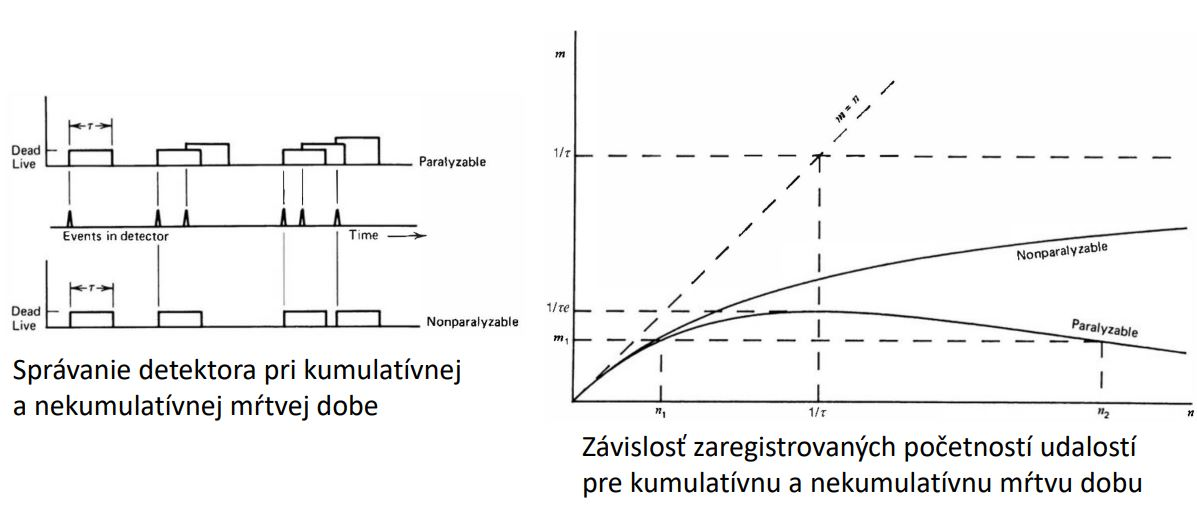
\includegraphics[width=0.8\textwidth]{img/mrtva_doba.JPG}
    \caption{Analýza mrtvé doby.}
\end{figure}

\textbf{Kalibrace detekční účinnosti:} ta není konstantní, je závislá na energii a typu záření. Je zapotřeba stanovit funkci detekční účinnosti za pomoci etalonů o známé aktivitě.

\begin{figure}[H]
    \centering
    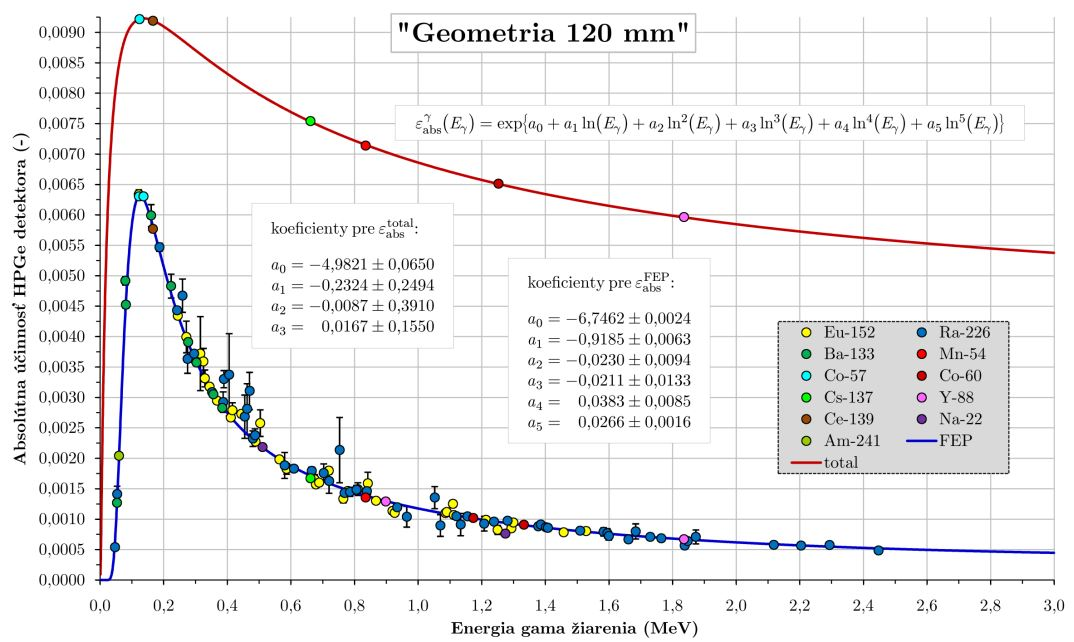
\includegraphics[width=0.8\textwidth]{img/detekcni_krivka.JPG}
\end{figure}

\textbf{Aplikace opravných faktorů:} na závěr je vhodné uvažovat opravné faktory:

\begin{itemize}
    \item oprava na RA rozpad (zářič se v průběhu měření rozpadá),
    \item oprava na nebodovost zdroje,
    \item oprava na samostínění (pro vzorky konečné tloušťky),
    \item oprava na náhodné koincidence (potlačení sumačních efektů).
\end{itemize}

Pak je možné určit finální aktivitu vzorku z analýzi FEP (v pořadí korekce na samostínění, korekce na rozpad a celková aktivita peaku):

$$ \boxed{ A = \dfrac{\mu L}{1 - e^{-\mu L}} \dfrac{\lambda t_\text{real}}{1 - e^{- \lambda t_\text{real}}} \dfrac{S}{I_\gamma \: \varepsilon_\text{FEP}^\text{abs} \: {t_\text{live}}}.} $$

